% !TEX encoding = UTF-8 Unicode
\RequirePackage{fix-cm}
\documentclass[a4paper,10pt,UTF8]{article}
%\documentclass[a4paper,10pt,UTF8]{ctexart}

\usepackage[english]{babel}
\usepackage{fancyhdr,array,lastpage,amsmath,amsfonts,mathtools,enumitem,graphicx,multirow,tocbibind,longtable,makecell,varwidth,titlesec,bm,booktabs,comment,todonotes,subcaption}
\usepackage{algorithm,algorithmic}
\usepackage{enumitem,supertabular}
\usepackage{datatool,filecontents}
\usepackage{hyperref,tablefootnote}
\hypersetup{hidelinks}
%\setCJKmainfont[BoldFont=Heiti SC Medium]{Songti SC Light}
%\setCJKsansfont{Heiti SC}

\usepackage[left=3.17cm,right=3.17cm,top=2.54cm,bottom=2.54cm]{geometry}
\usepackage[font=footnotesize,labelfont=bf]{caption}
\usepackage{tikz,flowchart}
\usetikzlibrary{shapes,shapes.geometric,arrows}
\usepackage{listings}
\usepackage[Q=yes]{examplep}
\usepackage{courier}
\usepackage[T1]{fontenc}
\usepackage{fbb}

\renewcommand{\dtldisplaystarttab}{\toprule}

% likewise for \midrule and \bottomrule from booktabs 
\renewcommand{\dtldisplayafterhead}{\midrule}
\renewcommand{\dtldisplayendtab}{\\\bottomrule}

\newcommand {\fd}{functional dependency}
\newcommand {\fds}{functional dependencies}
\newcommand {\funcdep}{$ \rightarrow $}
\newcommand {\mfuncdep}{ \rightarrow }
\newcommand {\mvd}{\mbox{$ \rightarrow \! \! \! \! \rightarrow  $}}
\newcommand {\mmvd}{ \mbox{\rightarrow \! \! \! \! \rightarrow }}
\newcommand {\md}{multivalued dependency}
\newcommand {\mds}{multivalued dependencies}
\newcommand {\fmds}{functional and multivalued dependencies}
\newcommand {\jd}{join dependency}
\newcommand {\jds}{join dependencies}
\newcommand*{\mat}[1]{\boldsymbol{\mathrm{#1}}}
\renewcommand*{\vec}[1]{\boldsymbol{#1}}

\newenvironment{sol}
  {\par\vspace{2mm}\noindent{\bf Solution}. }


\lstset{escapeinside=``, breaklines=true, frame=none, extendedchars=false, basicstyle=\ttfamily, showstringspaces=false}

\setlength{\parindent}{0em}
\setlength{\parskip}{1.5ex}
\linespread{1.1}

%\pagestyle{plain}
%\bibliographystyle{plain}

\numberwithin{equation}{section}
\numberwithin{figure}{section}

%\setcounter{secnumdepth}{3}
%\setcounter{tocdepth}{3}


\title{CS420 Machine Learning \\ Final Project}
\author{716030210013 \quad Mengyun Chen \\
716030210014 \quad Yuge Zhang}

\begin{document}

\maketitle

\renewcommand*\contentsname{Summary}

\tableofcontents


\everymath{\displaystyle}

\section{Introduction}

The requirement of the final project is to build a standard classifier for an ``non-standard version'' of MNIST dataset. It is also required to use at least \textbf{three} different approaches to complete the task.

In this report, we will first discuss the dataset, including how it is different from the standard version of MNIST dataset and what kind of information is useful in classification. Then we try some classic and simple approaches to address the issues. Some of them worked out; others didn't. Anyway, we will reach performance that is good enough (about 97\% to 98\%) with fewer than 100 lines of code and minutes of computing power on a laptop. For the last part, we will further implement the famous Variational Auto-Encoder, and some of its variations, as discussed in class. This neural network is capable of ``reconstruction'', which will further demonstrate the distribution of the data. The benchmark result and comparison between models that have been used in all these experiments are attached at the end of the report.

\section{Analysis}

\subsection{Dataset technical specifications}

\begin{description}
\item[Training sample size] 60000.
\item[Features] $45 \times 45$.
\item[Color] Grey. Integer range in $[0, 255]$.
\item[Labels] Integer in $[0,9]$.
\item[Test sample size] 10000.
\end{description}

\subsection{Difference from the standard version}

At first, we ran our tests on the standard version of MNIST, because somehow we couldn't download the dataset from the given address and therefore we assumed the dataset was exactly the same as the standard one. It wasn't until someone was starting to write the report that we discovered this little trick: \textbf{modified version}.

After reading the dataset and observe a few examples, we conclude that the modified version is actually modified in two ways:

\begin{enumerate}
\item The image is randomly extended with black blocks.
\item Some random noise has been added to the image.
\end{enumerate}

Note that we can use some preprocessing techniques to safely crack the first issue. That is, to locate the average / median position of the ``white'' pixels, and compute a $32 \times 32$ wrapper around this center. $32 \times 32$ is a little bit larger than the standard $28 \times 28$, but this is fine and it should leave some space for possible deviations.

Using 80 as threshold (pixels with values greater than 80 are considered as white), the program takes about 300 seconds to finish with \verb|numpy| implementation.

Let's call this process \textsc{Centering}. \autoref{fig:centering} shows how this procedure affects the image.

\begin{figure}[htbp]
\centering
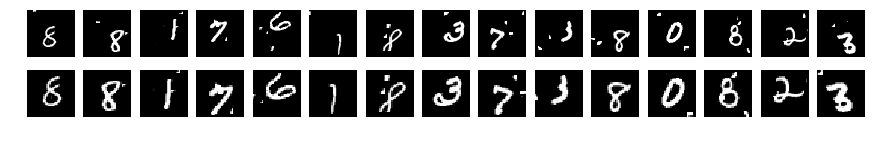
\includegraphics[width=1.0\textwidth]{img/centralize.png}
\caption{The upper row is for raw image. The bottom one is the processed.}
\label{fig:centering}
\end{figure}

\subsection{Hints from the legendary Homework 3}

This seems to be a standard classifcation problem, like many we have handled before which we can deal with using algorithms like SVM, kNN and similar. Homework 3 did offer us some hint on processing such tasks with sklearn library. We could simply copy the classifier ``template'' and modify some parameters and achieve not-bad results.

\paragraph{Thresholding} Not sure about the exact reason, but the intuition is that rounding the colors to only two: black and white, should help. (Maybe because it will help SVM build the gap since margin is always difficult for grey.) This is another preprocess step: \textbf{thresholding}. However, it turns out that this step is actually a trade-off. Benchmark results show that this intuition might be true for time usage, but not for accuracy. 

\paragraph{PCA with whitening} In homework 3, when dealing with the deep learning image recognition dataset, the unsupervised technique that uses PCA with whitening is used as a pre-step for the classification, and will contribute a lot to the performance: not only accuracy but also time usage. We will combine this technique with almost every method in this subsection.

\paragraph{kNN, SVM, MLP} We tried these three models with different combinations of methods mentioned above. kNN and SVM are very slow, and the performance is hardly satisfying. MLP is way much faster and the performance is not bad.

There is not much to discuss since the codes are all intuitively short. For now, we will not go into details, but later will discuss the comparisons between these traditional methods (maybe except MLP), and deep learning.

All experiment results are available in \autoref{benchmark}.

\subsection{Hints from Tensorflow tutorial}

Too many people have done too much research into MNIST dataset, so that the Tensorflow's tutorial for beginners is about MNIST...

Without GPU / TPU acceleration and little Tensorflow programming experience, training with Convolutional Neural Network seems to be both time consuming and unrewarding. With a modified version (only modified on the input data set size) of the CNN in the tutorial, we can only get accuracy less than 95\% with over an hour of training. Just for visualization purposes, we plot the cross entropy loss function with respect to training steps. See Figure \autoref{fig:cnn_loss}.

\begin{figure}[htbp]
\centering
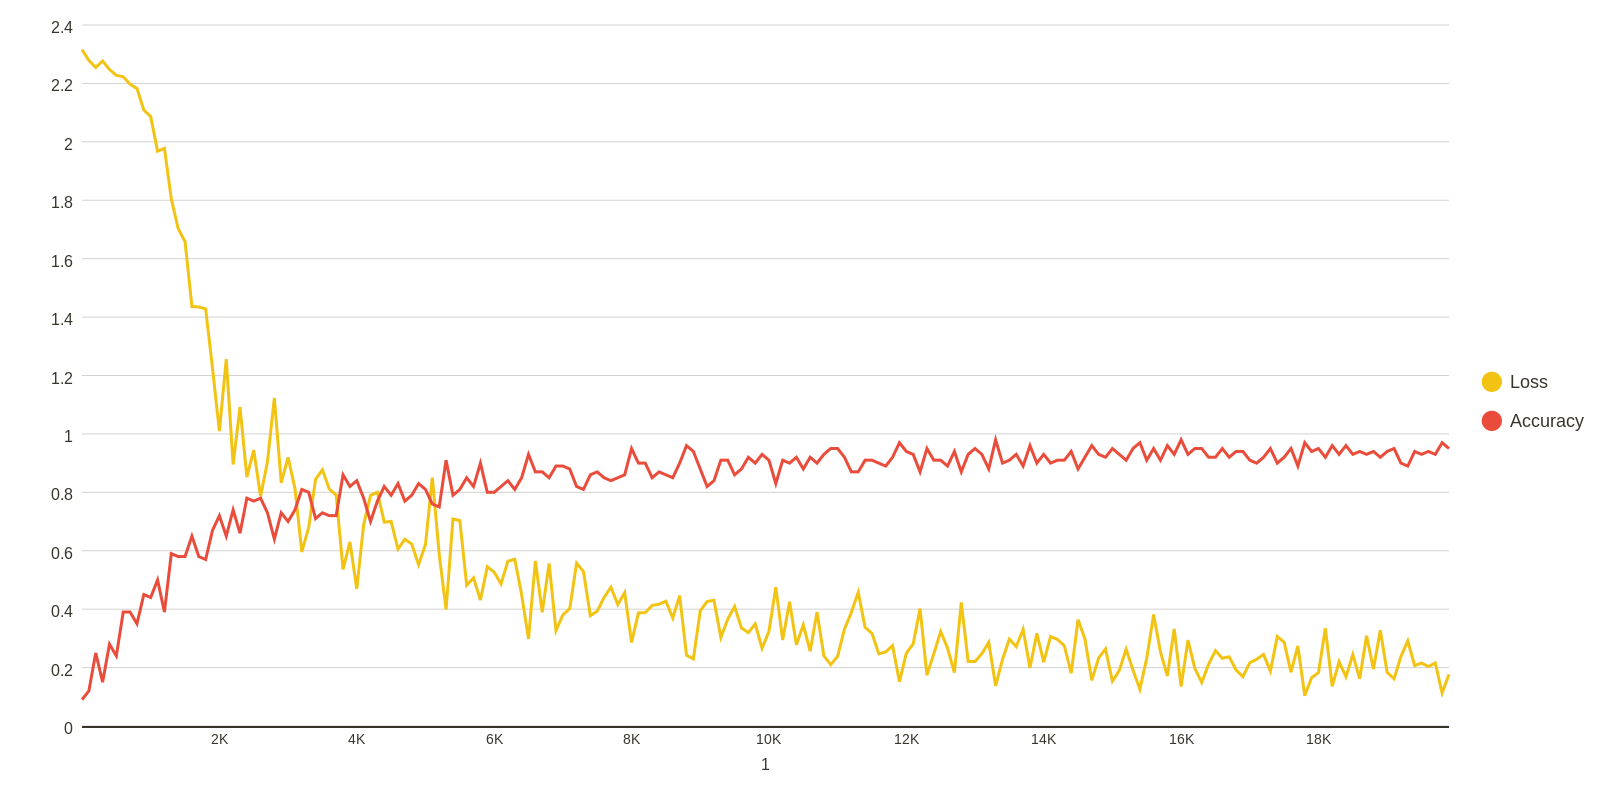
\includegraphics[width=1.0\textwidth]{img/cnn_loss.png}
\caption{CNN diagram. Generated by Tensorboard}
\label{fig:cnn_loss}
\end{figure}

\paragraph{A re-implementation} Actually, after we finish the part with Variational Auto Encoder, we re-implemented the CNN using Tensorflow low-level API. We omitted the dropout layer, for a mysterious belief that overfitting would accelerate the learning with almost little damage. The network structure is shown in \autoref{fig:cnn2diagram}.

\begin{figure}[htbp]
\centering
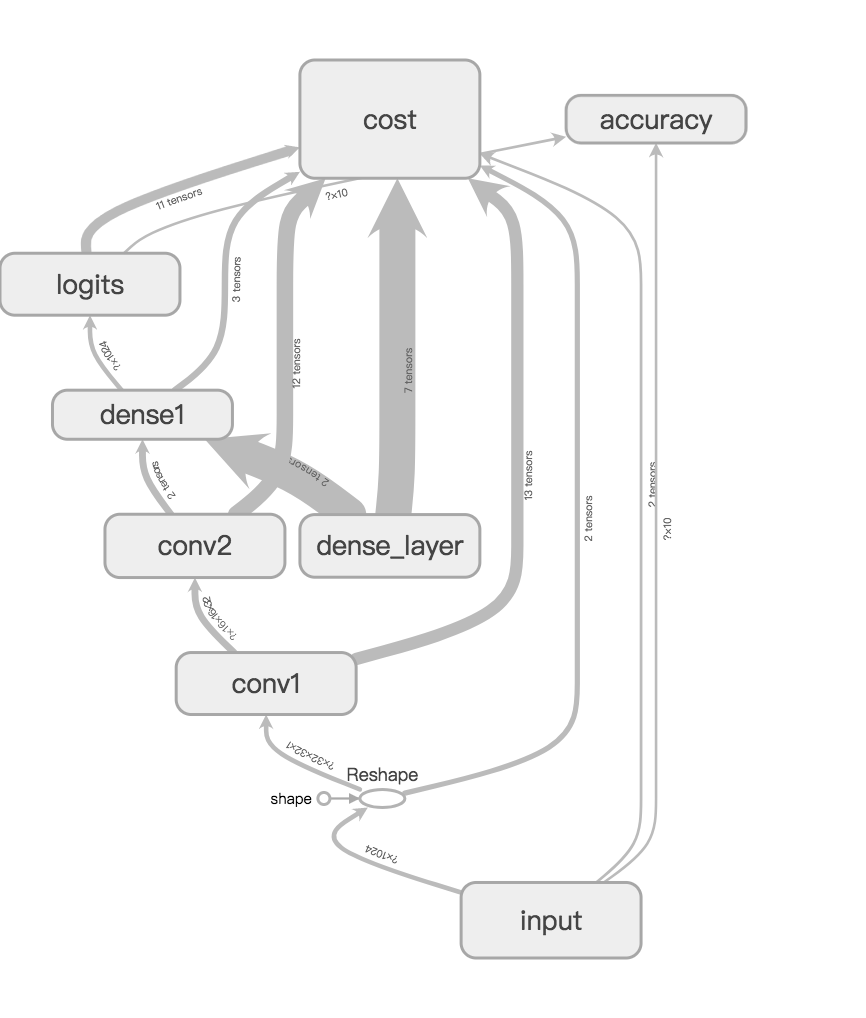
\includegraphics[width=0.5\textwidth]{img/cnn1.png}
\caption{CNN diagram. Generated by Tensorboard}
\label{fig:cnn2diagram}
\end{figure}

The experiment result with respect to training epochs is shown in \autoref{tab:cnn2}\footnote{This test uses the same machine as in the benchmark. See the benchmark section for details.}.

\DTLloadrawdb{cnn2}{csv/cnn2.csv}

\begin{table}[htbp]
\centering
\DTLdisplaydb{cnn2}
\caption{CNN varying epoch times}
\label{tab:cnn2}
\end{table}

It can be shown in the experiment result that the network has improved very little after epoch 3. For a deeper insight, we reduce the sample number of training data and see what effect it takes on the final result. The evaluation size is the same as before: 10000 samples. Now we have \autoref{tab:cnn2-sample}.

\begin{table}[htbp]
\centering
\begin{tabular}{ccccccc}
    \toprule
    \#samples & Epoch 1 & Epoch 2 & Epoch 3 & Final \tablefootnote{Epoch number and the final accuracy. Training quits if accuracy hasn't improved during last two epochs or it has reached 20.} & Total time \\
    \midrule
    1000 & 0.6431 & 0.7545 & 0.8087 & 6: 0.8374 & 18.8 \\
    2000 & 0.744 & 0.8617 & 0.9034 & 6: 0.9128 & 24.6 \\
    4000 & 0.8752 & 0.9251 & 0.9357 & 11: 0.9549 & 68.6 \\
    8000 & 0.9331 & 0.9474 & 0.9476 & 8: 0.9647 & 80.2 \\
    16000 & 0.9492 & 0.9597 & 0.9662 & 10: 0.9733 & 178.7 \\
    32000 & 0.9648 & 0.9729 & 0.9805 & 8: 0.9827 & 266.6 \\
    All & 0.9723 & 0.9802 & 0.9832 & 20: 0.9918 & 1219.5 \\
    \bottomrule
\end{tabular}
\caption{CNN varying training sample number}
\label{tab:cnn2-sample}
\end{table}

The convolution net is amazingly efficient and can reach about 93\% percent accuracy with sample size equal to the test sample size.

\section{Experiment with VAE}

\subsection{Variational Auto Encoder}

\subsubsection{Introduction}

Variational Auto Encoder, aka, VAE, is an unsupervised deep learning technique, that enables us to project the data into a latent space, and reconstruct our input using a sample in the latent space.

As VAE is unsupervised, it might be not intuitive to use VAE in a supervised labeling task. The reasons why VAE is introduced in this project are as follows:

\begin{enumerate}
    \item A step for dimension reduction; a substitute for PCA. Prepare for possible following supervised learning steps.
    \item Noise reduction. The input contains a lot of noise. Hopefully we can use reconstruction to remove those noise.
    \item Generate cool / fancy visualized facts about MNIST dataset.
\end{enumerate}

\subsubsection{Technical details}

Not sure about this part, but it seems important that we ``redefine'' some symbols here to make sure everything is clear.

We now have input $\vec{x}$. What VAE is trying to do is to find a latent variable $\vec{z}$ and reconstruct $\vec{x'}$. To make this happen, VAE builds two neural networks: encoder and decoder. For the decoder, VAE also assumes that $p(\vec{z} | \vec{x})$ is a multidimensional guassian distribution with mean $\mu(\vec{x})$ and variance $\Sigma(\vec{x})$; and the decoder part can be think of as a function that maps input $x$ into $\vec{\mu}$ and $\vec{\Sigma}$. For the decoder, we randomly sample a $\vec{z}$ from $\mathcal{N}(\vec{\mu}, \vec{\Sigma})$. And we apply a symmetircal network to compute $\vec{x'}$. Now comes the magical part, the loss function is computed as follows\footnote{Technically, we cannot subtract a vector from a number. This means we do the operation on every dimension. This is consistent with the implementation using Tensorflow.}:

\begin{equation}
    \textsc{ReconstrLoss} = \vec{x} \log (\vec{x'}) + (1 - \vec{x}) \log (1 - \vec{x'})
\end{equation}
\begin{equation}
    \textsc{LatentLoss} = - \frac{1}{2} (1 + \log(\det \mat{\Sigma}) - \mathrm{tr}(\mat{\Sigma}) - \vec{\mu}^T \vec{\mu})
\end{equation}
\begin{equation}
    \textsc{TotalLoss} = \textsc{ReconstrLoss} + \textsc{LatentLoss}
\end{equation}

For computational reasons, we denote the diagonal elements of $\mat{\Sigma}$ (those are the only non-zero elements) as a vector, and use the logarithm of the vector as the dense layer output.

A demo visualization of VAE is shown in \autoref{fig:vae1}. This demo  has three dense layers each as decoder and encoder. 

\begin{figure}[htbp]
\centering
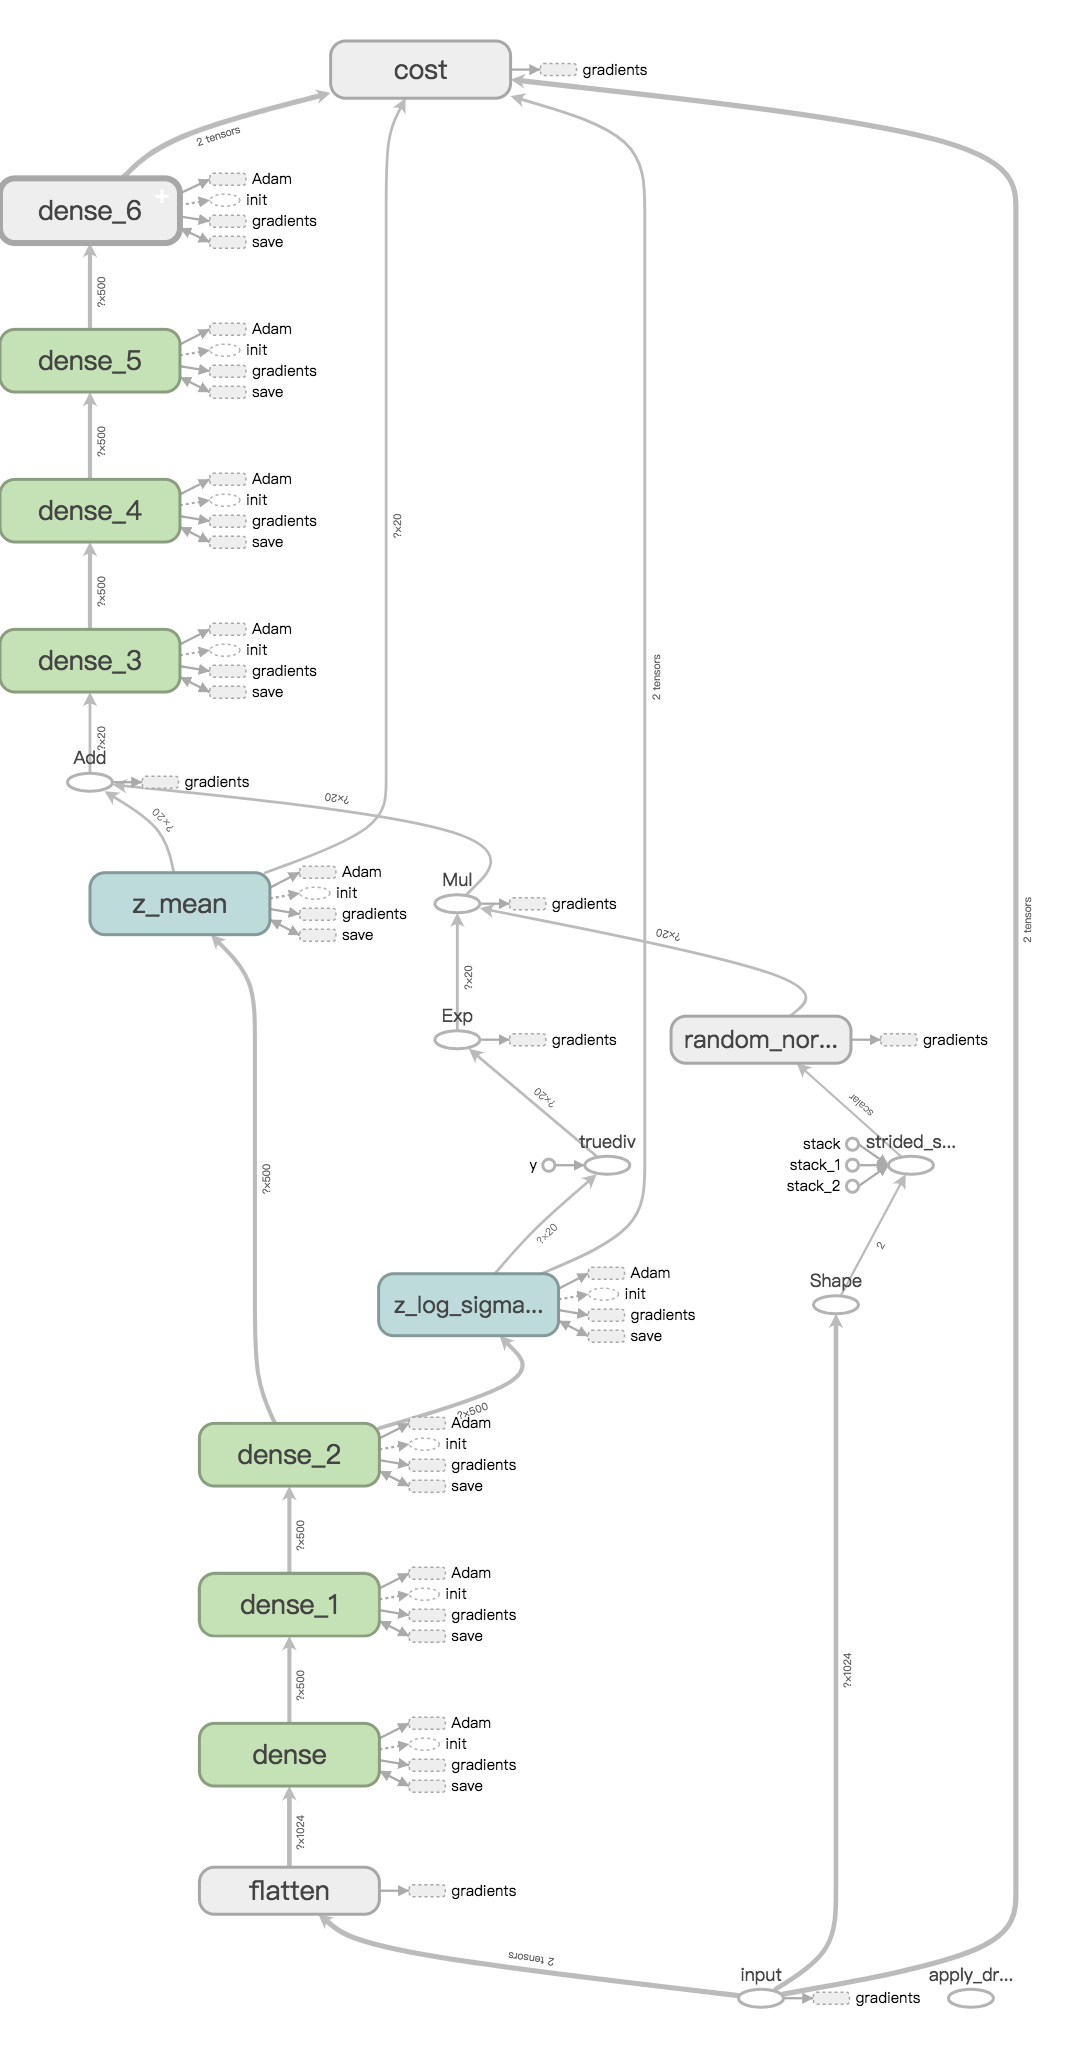
\includegraphics[width=0.8\textwidth]{img/vae1.png}
\caption{VAE diagram. Three layers each. Generated by Tensorboard}
\label{fig:vae1}
\end{figure}

\subsubsection{Dimensionality reduction (vs. PCA)}

How does VAE perform in reducing dimensions? To visualize the performance, we set the dimension of $\vec{z}$ to be 2. In this experiment, we set epoch to be 50. The training takes about 4 minutes. \autoref{fig:vae_vs_pca_dimreduce} shows the scatter plot. It's the immediate fact from the plot that VAE seems to be more scattered.

\begin{figure*}[htbp]
    \centering
    \begin{subfigure}[h]{0.49\linewidth}
        \centering
        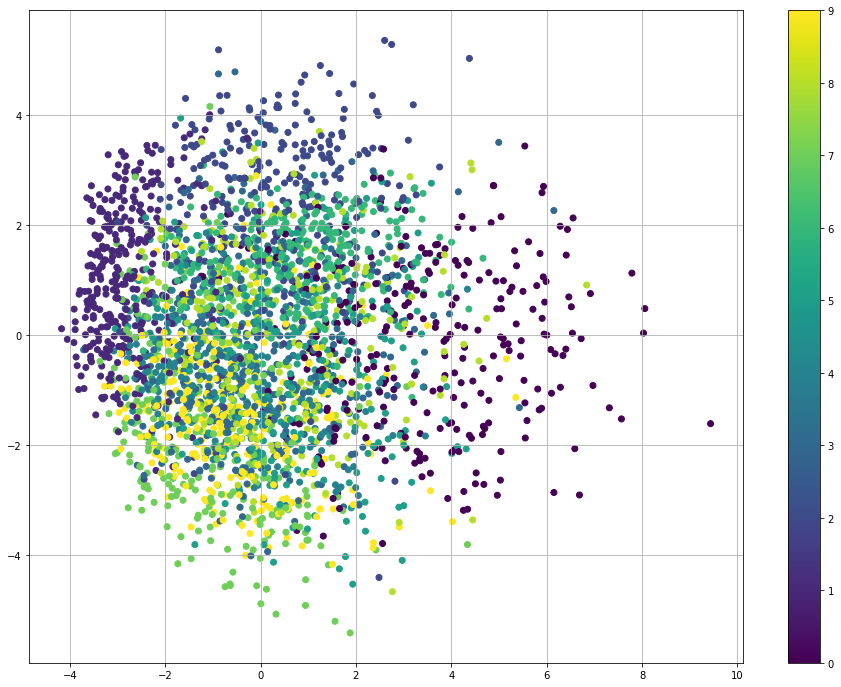
\includegraphics[width=1.0\textwidth]{img/dimreduce_pca.png}
        \caption{Result with PCA}
    \end{subfigure}
    \begin{subfigure}[h]{0.49\linewidth}
        \centering
        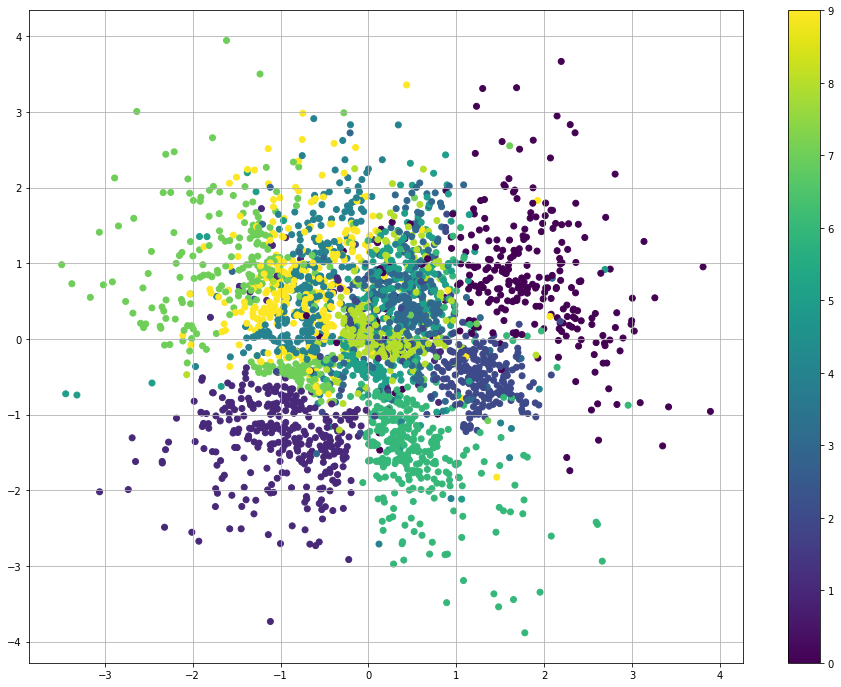
\includegraphics[width=1.0\textwidth]{img/dimreduce_vae.png}
        \caption{Result with VAE}
    \end{subfigure}
    \caption{Dimensionality reduction performance comparison}
    \label{fig:vae_vs_pca_dimreduce}
\end{figure*}

Here is something that PCA is unable to do: reconstruction. We iterate over $\vec{z} = [z_1,z_2]^T$ for $2.5 \le z_i \le 2.5$, and we get \autoref{fig:vae_reconstr_2d}\footnote{This figure is inversed in color for better outlook on a white sheet}. The image looks very blurry, especially on the border. And some numbers like 5 and 9, takes very little space before it blends in with others. We will see that this actually brings difficulty to the classification task in the next section.

\begin{figure}[htbp]
\centering
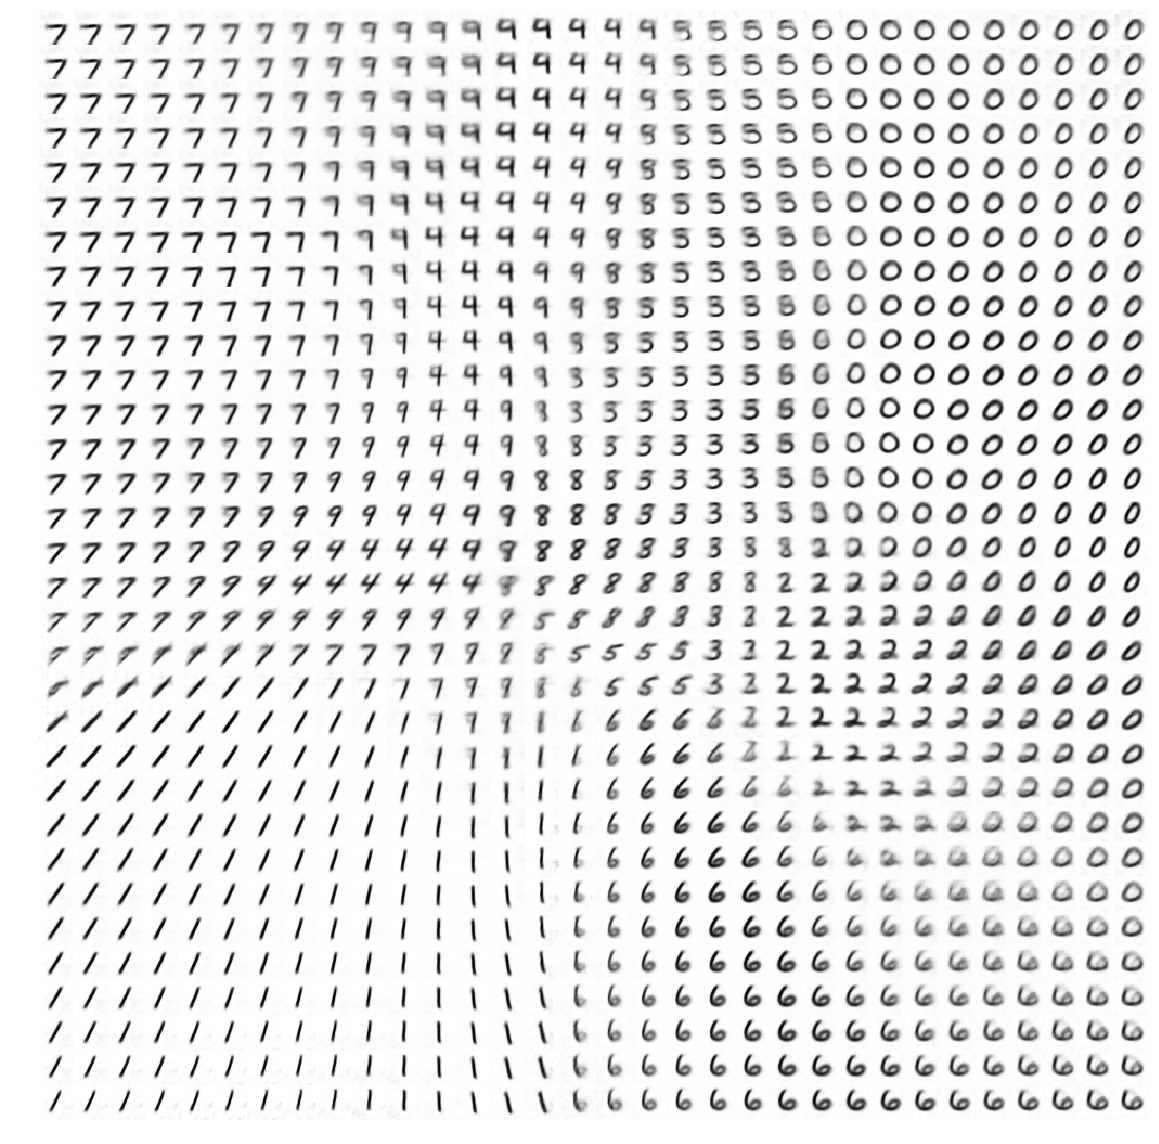
\includegraphics[width=0.6\textwidth]{img/reconstr_2d.png}
\caption{VAE 2D reconstruction}
\label{fig:vae_reconstr_2d}
\end{figure}

\subsubsection{Work with CNN}

Combining CNN with VAE, we use ``conv'' in the encoder layers, and ``deconv'' in the decoder layers, we can get the structure as shown in \autoref{fig:convnet_structure}.

\begin{figure}[htbp]
\centering
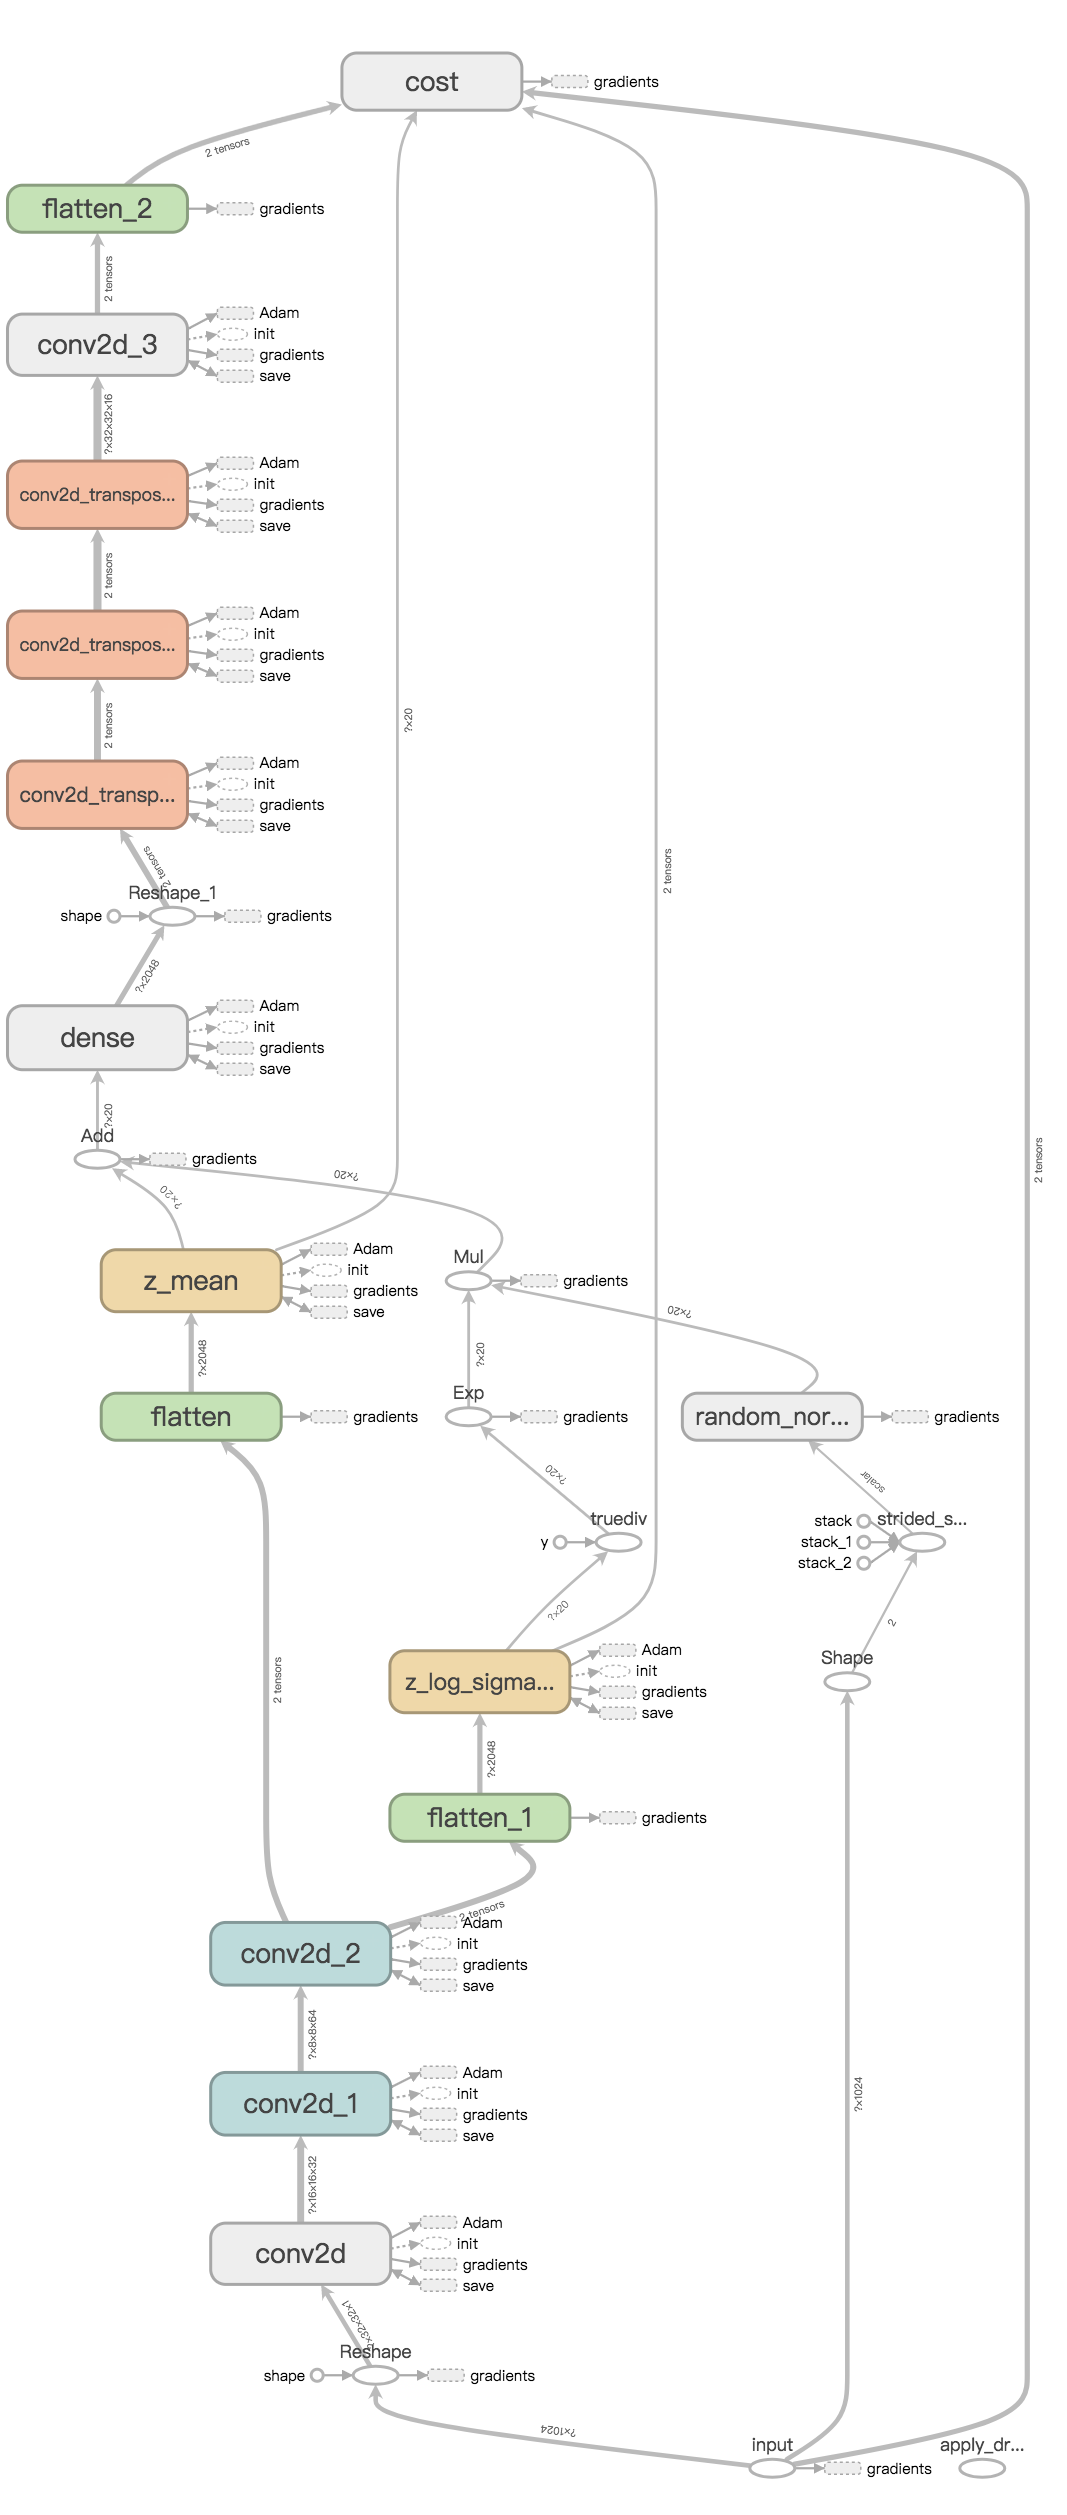
\includegraphics[width=0.7\textwidth]{img/convnet_structure.png}
\caption{VAE with CNN. Generated by Tensorboard}
\label{fig:convnet_structure}
\end{figure}

How well is the performance of this network? We tried to apply some reconstruction on some randomly picked test data, as shown in \autoref{fig:reconstr_compare}. We can see that this is even sharper than standard-dense-layered VAE. Also notice that the reconstruction network already make assumptions, for example, the 5 is believed to be 6. Although, currently the network knows nothing about what is 5 or what is 6. Also, compared to PCA, who is doing linear transformation as usual, VAE generally has less distortions.

\begin{figure}[htbp]
\centering
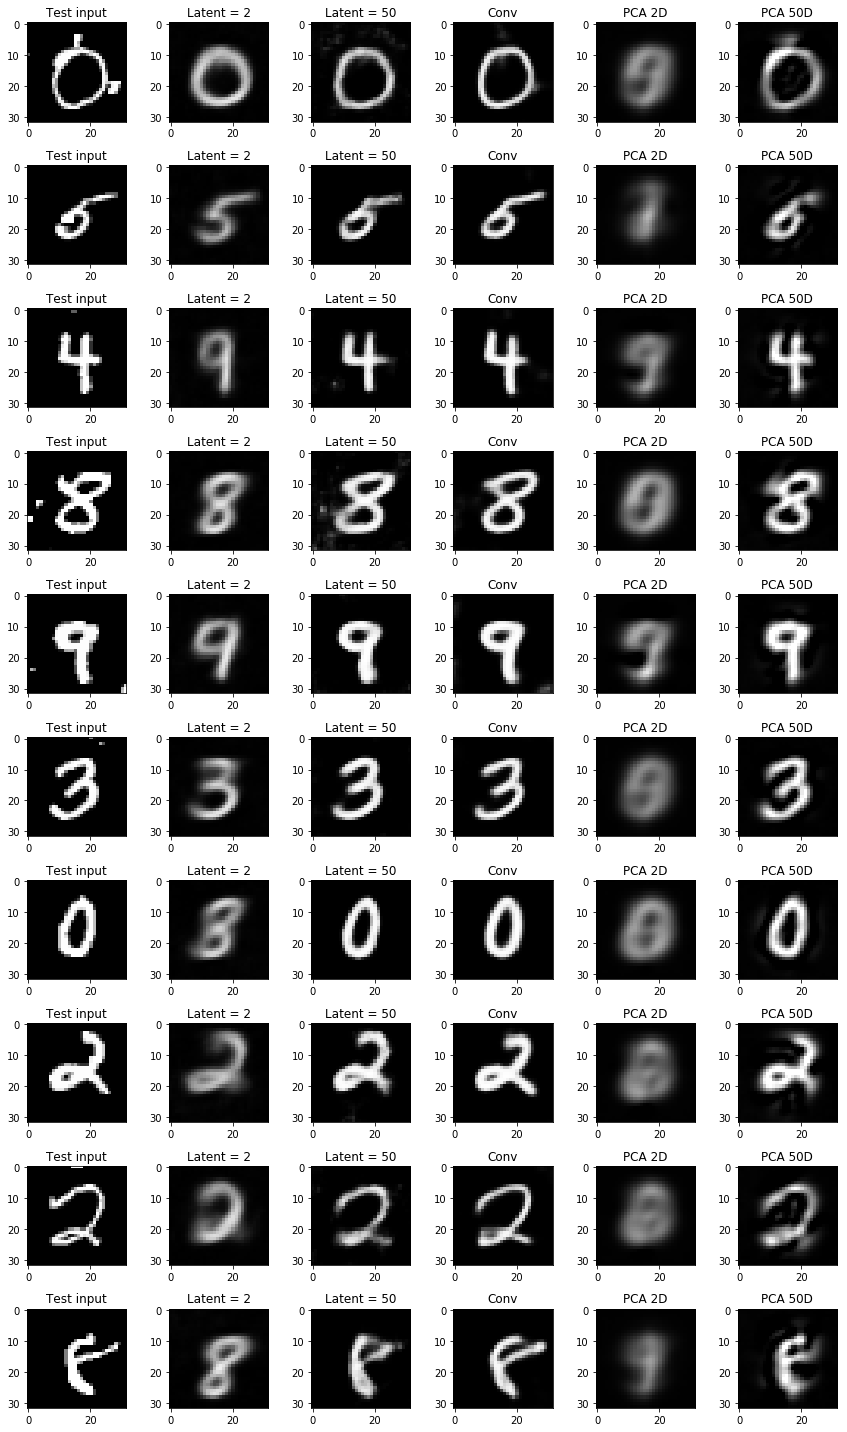
\includegraphics[width=0.7\textwidth]{img/reconstr_compare_pca.png}
\caption{VAE / CNN / PCA. Comparison}
\label{fig:reconstr_compare}
\end{figure}

\subsubsection{Classification}

It might be disappointing that when we actually use the latent variable $\vec{z}$, with SVM, to do the classification, the performance does not even outcompetes the simple method using PCA + SVM. Even using a convolutional VAE that has been trained for about 8 hours, the accuracy is 0.9634 -- still a little bit less than the model with PCA. We tried to improve this with the information provided in the confusion matrix, but hardly helpful.

$$
\begin{bmatrix}
 977 &    1 &    0 &    1 &    0 &    2 &    7 &    1 &    1 &    2 \\
   0 & 1177 &    5 &    2 &    0 &    0 &    2 &    5 &    2 &    0 \\
   1 &    3 & 1001 &    2 &    3 &    3 &    1 &    6 &    9 &    2 \\
   0 &    0 &   14 &  977 &    1 &   12 &    3 &    3 &   15 &    5 \\
   1 &    3 &    3 &    0 &  887 &    0 &    4 &    6 &    1 &   22 \\
   2 &    1 &    1 &   16 &    0 &  849 &   12 &    0 &   10 &    3 \\
   4 &    3 &    0 &    3 &    3 &    5 & 1001 &    0 &    1 &    1 \\
   2 &    5 &    8 &    4 &    9 &    1 &    1 &  978 &    0 &   20 \\
   2 &    2 &    4 &   12 &    2 &    8 &    3 &    4 &  875 &   10 \\
   3 &    1 &    2 &    2 &   17 &    3 &    2 &   14 &    6 &  912
\end{bmatrix}
$$

It's not intuitive why reconstruction of VAE seems to be look better but performs badly on the classification task. One possible reason is that the information machines need for classification is not exactly the information that is needed for reconstructing human-friendly images. 

\subsection{Conditional Variational Auto Encoder}

Conditional VAE is not a new concept. In short, it modifies VAE by encoding $[\vec{x},\vec{y}]$ instead of $\vec{x}$, and decoding $[\vec{z},\vec{y}]$ instead of $\vec{z}$.

Again, out of the mysterious belief that $\vec{y}$ should not go into some uncontrollable network, we first added $\vec{z}$ at the last layer, that is, the layer to calculate the mean and variance of $\vec{z}$, instead of concatting the vectors before everything. Later we found that feeding $\vec{z}$ into every layer would possibly do better -- this would, intuitively, increase the degree to which labels matter.

Due to lack of reference, building a CVAE is completely out of intuition and experimental feedbacks. We add some dropout layers to prevent overfitting. The whole network structure is shown as in \autoref{fig:cvae_structure}.

\begin{figure}[htbp]
\centering
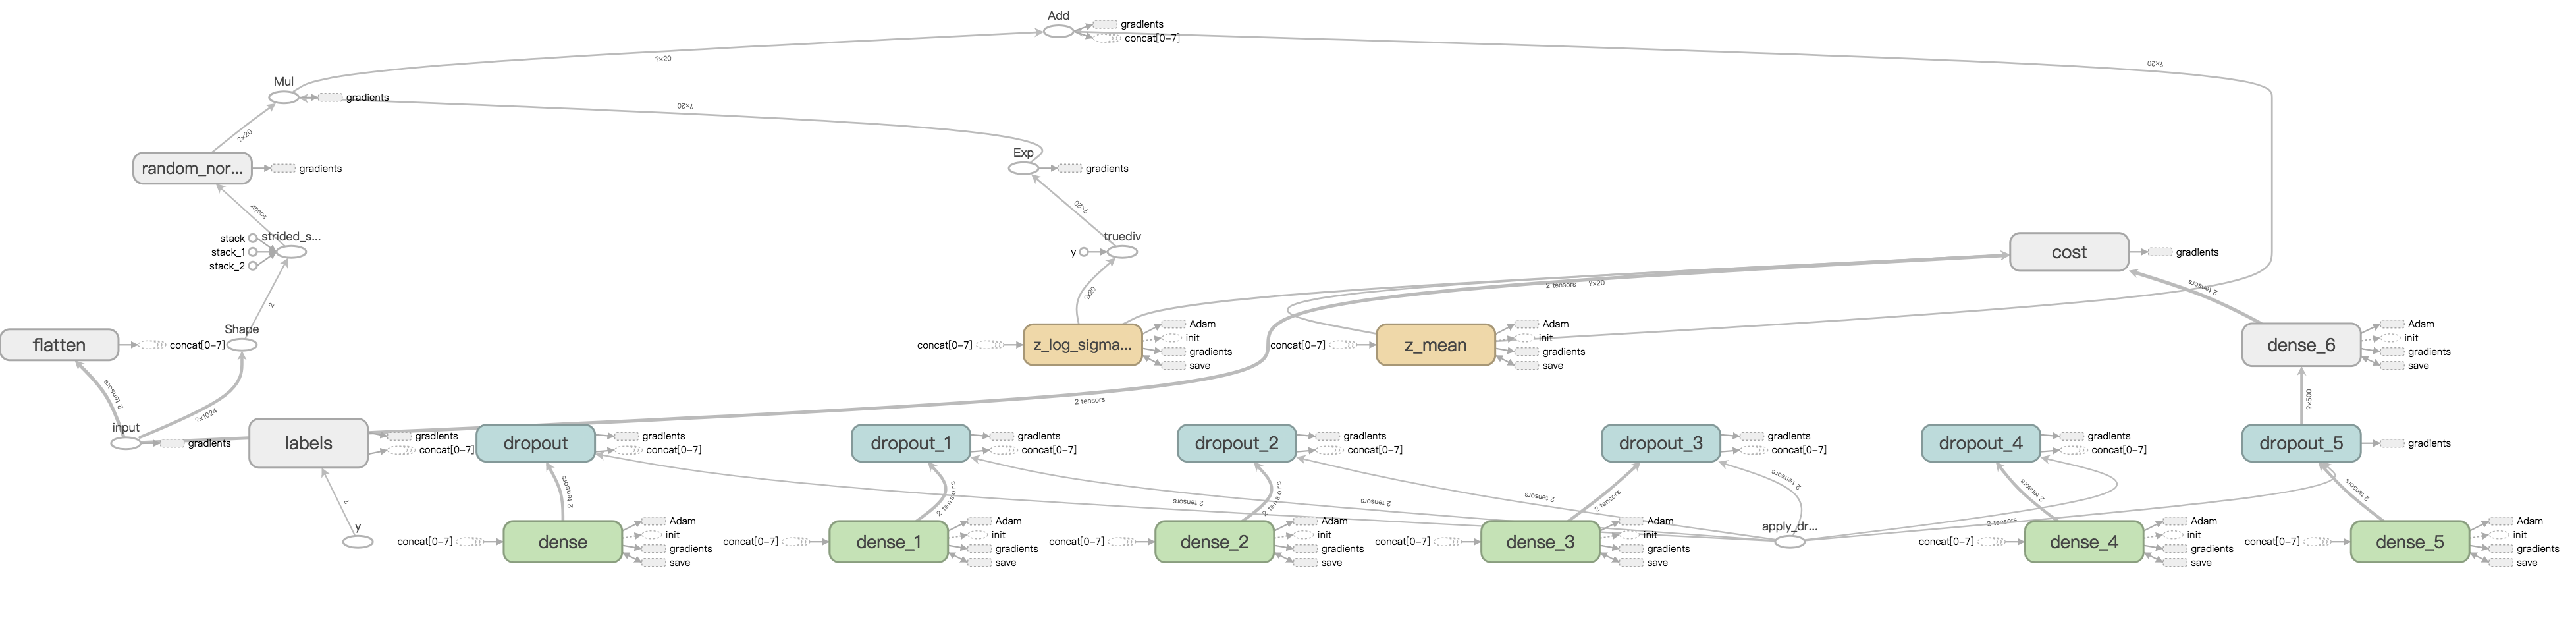
\includegraphics[width=1.0\textwidth]{img/cvae_structure.png}
\caption{CVAE. Generated by Tensorboard}
\label{fig:cvae_structure}
\end{figure}

A representative application of CVAE is that we can control the label and generate different styles of a number, as shown in \autoref{fig:cvae_style_generation}.

\begin{figure*}[htbp]
    \centering
    \begin{subfigure}[h]{0.49\linewidth}
        \centering
        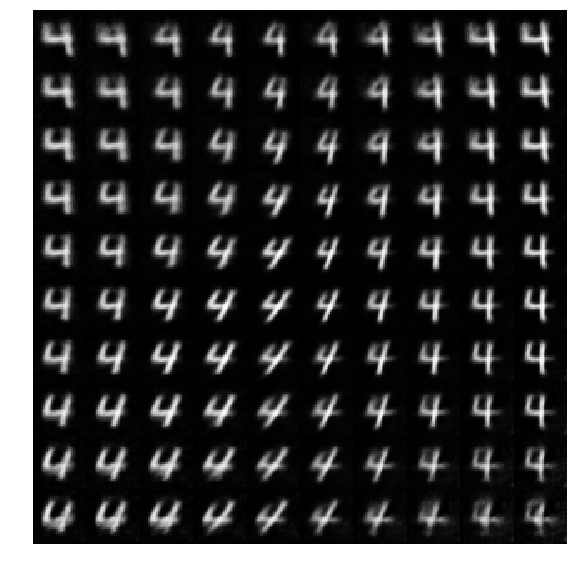
\includegraphics[width=1.0\textwidth]{img/cvae_4.png}
        \caption{Different styles of 4}
    \end{subfigure}
    \begin{subfigure}[h]{0.49\linewidth}
        \centering
        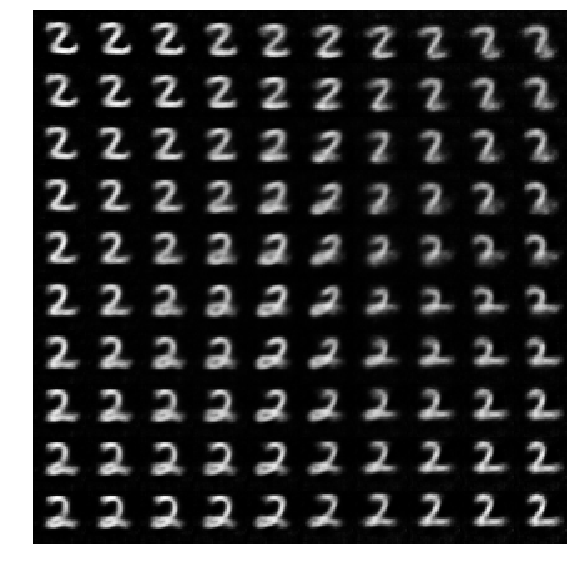
\includegraphics[width=1.0\textwidth]{img/cvae_2.png}
        \caption{Different styles of 2}
    \end{subfigure}
    \caption{CVAE generates different styles of numbers}
    \label{fig:cvae_style_generation}
\end{figure*}


How exactly does CVAE help in classification? Note that what CVAE is good at, is also reconstruction. The advantage is it can generate the answer given a label. Therefore we can guess a label and use the guessed label and raw image to reconstruct a new image. We calculate the reconstruction loss to determine which guessed label will give us the minimum loss. The algorithm pseudo code is demonstrated in Algorithm \ref{alg_cvae}.

\begin{algorithm}  
\caption{\textsc{Predict}($x$)}
\label{alg_cvae}
\begin{algorithmic}
\REQUIRE{$\vec{x}$ is a $n$-dimension vector.}
\FORALL{$y$ in $[0,9]$ \AND $y$ is an integer}
    \STATE regenerate $\vec{x'}$ with $(\vec{x}, y)$.
    \STATE \textsc{BestLoss} $\leftarrow \infty$
    \IF {\textsc{ReconstrLoss}$(\vec{x}, \vec{x'})$ $<$ \textsc{BestLoss}}
        \STATE \textsc{BestLoss} $\leftarrow$ \textsc{ReconstrLoss}$(\vec{x}, \vec{x'})$
        \STATE \textsc{Label} $\leftarrow y$
    \ENDIF
\ENDFOR
\RETURN \textsc{Label}
\end{algorithmic}
\end{algorithm}

\autoref{fig:cvae_reconstr} shows the reconstruction of the image using labels from 0 to 9.

\begin{figure}[htbp]
\centering
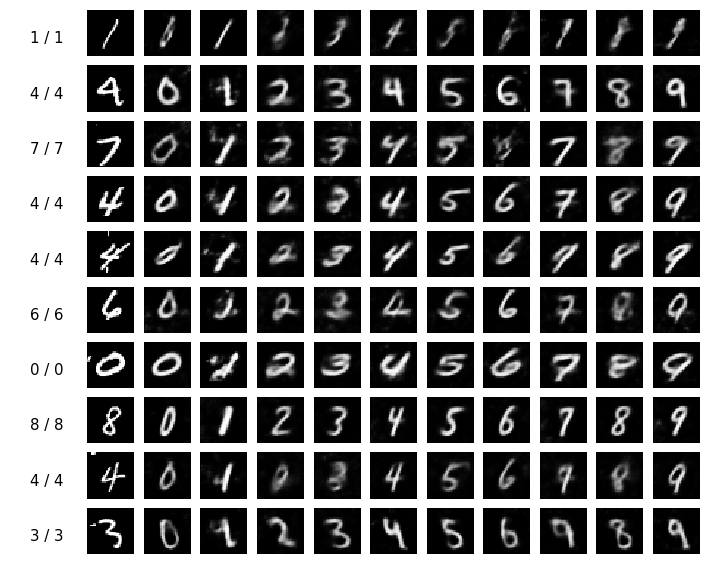
\includegraphics[width=0.8\textwidth]{img/cvae_reconstr.png}
\caption{CVAE reconstruction with label from 0 to 9}
\label{fig:cvae_reconstr}
\end{figure}

The reconstruction effect seems reasonably okay, it also helps \textbf{denoising}: you can see almost all the noises in the input image has been magically removed; but the accuracy is relatively low (less than 95\%). To investigate the reason, we tried to plot the reconstruction details of the images that are predicted incorrectly. This is \autoref{fig:cvae_reconstr_error}.

\begin{figure}[htbp]
\centering
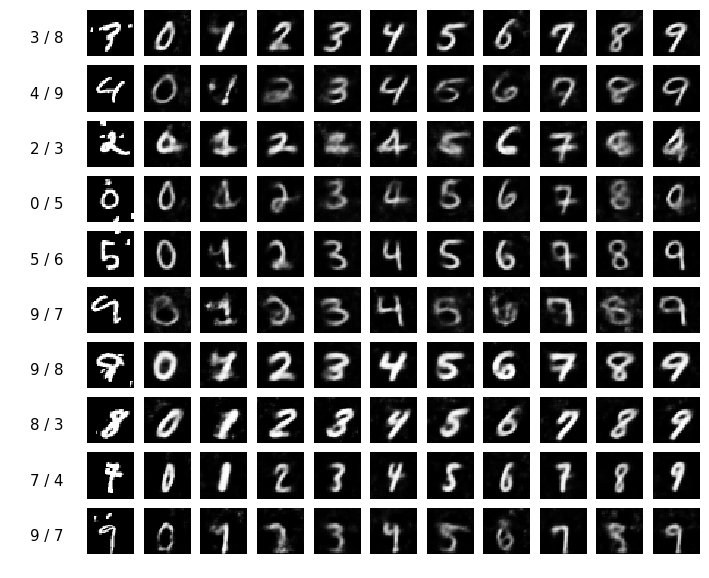
\includegraphics[width=0.8\textwidth]{img/cvae_reconstr_error.png}
\caption{Errors from the first 200 samples}
\label{fig:cvae_reconstr_error}
\end{figure}

It seems that the image is reconstructed ``incorrectly'' because they are adjusted to average shape during the reconstruction, which results in the deviation from the raw image data. The key idea why this algorithm should work is the belief that when using the correct label, the input image will not change much. As a matter of fact, these images did not change much in the shape, but in terms of the loss function, someone else, with a different shape, outcompetes them.

Now we had no clue about how to solve this problem, and had to give up.

\paragraph{NOTE} We suffer strange issue that the cost will be NaN after dozens of epochs. We didn't solve the problem, but used the checkpoint to restore the latest useful version.


\section{Benchmark}

\label{benchmark}

The benchmark test is done on a server with Intel Xeon CPU E5-2650 v4 @ 2.20GHz with 24 cores and 32 GB RAM, without GPU.

The time is not actually the CPU time usage, but the real time usage, because parallelism of the program is also an important metrics. We don't consider it a burden if a program uses more cores than another one. Also notice that the time includes training time and evaluation time. (Intuitively, kNN is slow because it has long evaluation time.)

The benchmark is grouped into 3 parts, which correspond to: traditional methods, CNN and VAE. In the ``traditional'' group, SVM + PCA is the best method. We get approximately 96.8\%, which is better than all the attempts with VAE. CNN gives us the global best, about 99.1\%. It might be surprising that the autoencoder group performs poorly in classification. However, autoencoders might be able to give us more knowledge than simply classify them. We can even denoise the images using CVAE.

The full benchmark is shown in \autoref{tab:benchmark}.

\begin{table}[htbp]
    \centering
    \begin{tabular}{ccccc}
    \toprule
        Method & Preprocess & Accuracy & Time (second) & Comment \\
    \midrule
        MLP & None & 0.6027 & 296.6 & iter = 101 before converge \\
        MLP & Centering & 0.8908 & 79.0 & iter = 48 before converge \\
        MLP + PCA \footnote{whitening is enabled by default for all PCA in tests} & None & 0.8372 & 100.6 & iter = 165 \\
        MLP + PCA & Centering & 0.9432 & 112.7 & iter = 198 \\
        kNN & Thresholding & 0.7057 & 368.5 & eval time is 332.5 \\
        kNN & Centering & 0.9306 & 196.9 & eval time is 160.8 \\
        kNN & Thres + Cent & 0.9011 & 161.3 & eval time is 124.4 \\ 
        SVM + PCA & Thresholding & 0.882 & 353.3 & \\
        SVM + PCA & Centering & \textbf{0.9678} & 144.1 & \\
        SVM & Thres + Cent & ? & $\infty$ \tablefootnote{We failed to wait for the result.} & \\
        SVM + PCA & Thres + Cent & 0.9641 & 147.4 & \\
    \midrule
        CNN (TF Demo) & Centering & 0.9481 & 3606.9 & step = 20000 \\
        CNN & Centering & 0.9723 & 57.9 & epoch = 1 \\
        CNN & Centering & 0.9832 & 178.8 & epoch = 3 \\
        CNN & Centering & \textbf{0.9905} & 1219.5 & epoch = 200 \\
    \midrule
        VAE + SVM & Centering & 0.6944 & $\approx$ 400 & latent dim = 2 \\
        VAE + SVM & Centering & 0.9403 & $\approx$ 600 & latent dim = 50 \\
        VAE (Conv) + SVM & Centering & 0.9634 & $\approx$ 8 hours & \\
        CVAE & Centering & 0.9423 & 1297.5 & \\
    \bottomrule
    \end{tabular}
    \caption{Benchmark result}
    \label{tab:benchmark}
\end{table}


\section{Conclusion}

This section is intentionally left blank.

\section{Code Repo}

The code repository is available at \url{https://github.com/ultmaster/MNIST-Toy-Machine}.

Since we have too many unsuccessful attempts. all the ``ridiculous'' models, even those that have possibly been mentioned in this report due to their nonsense, have been moved to the \verb|old| directory. There is also a notebook directory, containing the drafts, visualization code, and some other surprises. (It contains a lot of chaos; you may not want to check that.)


\end{document}
